\chapter{Firefox Add-on Development}

An add-on is a piece of software that augments another application. Based on the browser, different terms are used to refer to this software, like add-on, plug-in, or extension. An add-on cannot be executed as stand-alone software. Add-ons are used for different purposes like blocking advertisements and popups, downloading videos, and also to integrate several social network sites. 

Below are some of the applications of add-ons
\begin{enumerate}
\item An add-on can change the browser interface, which includes changing themes, the look and feel of buttons, the menu bar, and tabs.
\item They are also capable of adding new features to the browser, like providing easy usage of various softwares in the form of toolbars. 
\item Add-ons can also modify the behavior of browsers, like customizing the search option or page redirection. 
\item Add-ons used as plug-ins let the browser support internet content. These include Flash, Silverlight, and music players like QuickTime, real player, online games, and many more. 
\item On many browsers, online privacy is protected using add-ons. There are many types of add-ons that help to control and secure browsing and avoid attacks like preventing the user movements tracking on the browser.
\end{enumerate}

Browser Extensions are supported by Microsoft Internet Explorer starting with version 5 released in 1999. From 2004, Mozilla Firefox supports add-ons [37]. The Opera browser supports extensions starting with the desktop version 10 which was released in 2009. Google Chrome and Safari added support for extensions in 2010. Each browser has different variations in the browser extension syntax and they are compatible to their browser alone i.e., an extension built for one browser doesn`t work on another. For using search engine tools irrespective of browsers, a project named `Mycroft' [37] has been proposed, which is a database of over 20,000 search engine add-ons supported by multiple browsers.

\section{Firefox vs Chrome} 

In new era, out of all the browser extensions, Firefox and Chrome are most well known because of their popularity, security, and appearance. Below are some of the notable comparisons between them regarding extensions: 
\begin{enumerate}
\item Firefox has an outstanding extension base, i.e., https://addons.mozilla.org/en-US/firefox/, that offers more capable add-ons compared to all other browsers [39]. 
\item Firefox add-ons are very powerful and can perform anything that a Firefox process allows. Security features can be integrated into a Firefox add-on in a much more effective manner than Chrome extensions. So, it is possible to develop more advanced add-ons in Firefox, which would not be achievable on different browsers. Unlike Firefox, Chrome does not trust extensions completely and they provide very constrained APIs. For instance, without the user`s approval, extensions in Chrome can`t access the resource present outside of Chrome`s sandbox, but a Firefox add-on can access the resource in the filesystem without the user`s permission. 

For example, even though there are many Chrome extensions like ScriptSafe, NoScript Lite, which are similar to Firefox's "NoScript", till now no chrome extension is able to provide all the features of Firefox's NoScript because of the Chrome's constrained extension APIs.
\item By providing constrained extension APIs, Chrome presents a permission system and restricts its extensions a bit more for security. Whereas in Firefox, as the add-ons has more privileges, there are chances of infecting a victim`s machine. At worst, we may have to re-install the operating system to undo the effect created by a malicious add-on. To avoid these potential issues and to ensure that the add-ons are safe to install, they are manually reviewed before they publicly appear in the Mozilla add-ons gallery.
\end{enumerate}

To detect JavaScript malware, we have to generate opcodes for the JavaScript code in the webpage and to save these opcodes we may need access to the user`s filesystem and also we need to execute some other external scripts to validate the JavaScript code based on the saved opcodes. These tasks are only possible with the powerful APIs provided by Firefox, so we decided to implement a Firefox add-on to detect metamorphic malware.
\section{SDK vs XUL} 

There are two main ways to build Firefox extensions. The traditional way is using XPCOM (Cross Platform Object Model) and XUL (XML User Interface Language). Much of Mozilla`s documentation is focused on XUL add-ons, because this has been around for many years. More details about XUL add-on development can be found at [32]. The add-on SDK is the newer kind and was built under the Jetpack Project. Jetpack`s main agenda is to make it easy to build Firefox add-ons by using HTML, CSS, and JavaScript [3].

It is advisable to use the Add-on SDK because of the advantages it provides compared to XUL [33]:

\begin{enumerate}
\item Simplicity: High-level JavaScript APIs provided by the SDK like basic user interface components and their functionality simplify all the common tasks in add-on development. 
\item Compatibility : Electrolysis [34], also called e10s, is the project under which Firefox is being developed with a new multiple process architecture. The API`s provided by this SDK are designed to be forward-compatible with this new architecture. 
\item Security: It is not easy to build insecure add-ons using the SDK. Even the insecure Add-on that was compromised can do much less damage to the victim`s machine.
\item No restarts required: To install extensions developed using the SDK, we do not need to restart the browser.
\item Mobile Support: Add-ons can be developed for Firefox mobile using the experimental support provided by SDK 1.5
\end{enumerate}

However, XUL provides a huge number of options for the UI when compared to the SDK, and that`s the reason XUL is used for developing add-ons that require a rich user interface.

In this research, all the add-ons are built using the SDK as it provides simple APIs for developing most of the common tasks.

\section{Chrome Authority Usage}

Chrome Authority has nothing to do with Google Chrome. The Mozilla Developer Network(MDN) defines "\textbf{chrome}" as any visible parts of a browser other than the web pages, For instance, tabs, menu bar, and toolbars.

From the beginning of developing the SDK, it was assumed that developers may need to access the underlying browser (or) XPCOM services. So, the add-on SDK was developed to provide "chrome privileges" to the most powerful low level APIs. The "chrome privileges" grants low-level APIs to access the Components object that gives unrestricted access to the user system.  

With chrome privileges, an add-on can perform any function the browser is capable of. These privileges can be obtained by the add-on using the "chrome" module as shown below [1]:
\begin{lstlisting}[frame=single,language=JavaScript,numbers=none,mathescape=false]
var {Cc, Ci} = require("chrome");
\end{lstlisting}
The "chrome" module returns a Components object, which can be unpacked using the destructuring assignment feature provided by Mozilla JavaScript to obtain the Components.* aliases: 
\begin{enumerate}
\item Cc, otherwise called Components.classes
\item Ci, otherwise called Components.interfaces
\item Cu, otherwise called Components.utils.
\item Cr, otherwise called Components.results.
\item Cm, otherwise called Components.manager.
\end{enumerate}
It is not advisable to use chrome authority in the add-on code unless it is required because the add-ons that uses chrome authority require extra security review before they are made available for distribution to the public.

\section{Content Scripts} \label{sec:contentscript}

The add-on`s main code, including "main.js" and other modules in "lib", can use the SDK high-level and low-level APIs, but can`t access web content directly. Whereas content scripts can`t use the SDK`s APIs, but can access web content.

So if we have to build an Add-on that works based on the content of the web page, then we have to make use of the content scripts to access the web page contents. Content scripts are placed in the data subdirectory and they can be loaded into Add-on using contentScript or contentScriptFile option.

\textbf{Communicating with the add-on:}

To enable add-on scripts and content scripts to communicate with each other, each end of the conversation has access to a port object.
\begin{enumerate}
\item port.emit() is used to send messages from one side to the other 
\item port.on() is used to receive messages sent from the other side
\end{enumerate}

\begin{figure}
  \centering
      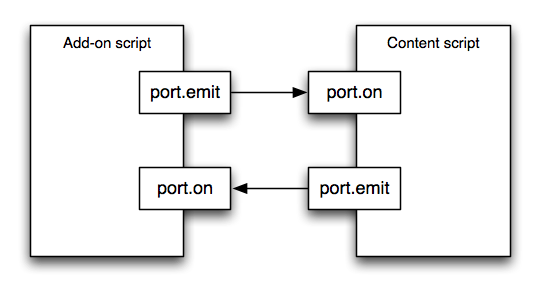
\includegraphics[width=16cm, height=8.65cm]{content-scripting-overview.png}
    \caption[Communication among add-on and content script]{Communication among add-on and content script [1].}
    \label{fig:content-scripting-overview}
\end{figure}

Messages are asynchronous i.e., after sending the message, sender continues processing without waiting for a reply from the recipient.

The add-on code in Figure~\ref{fig:communication} adds a button to Firefox. When the user clicks this button, add-on attaches a content script to the active tab, sends the \textbf{addon-message} to content script. When content script receives add-on message, it will retrieve the first paragraph from the loaded web page and send it to add-on along with \textbf{script-response} message. As soon as the add-on receives a response from content script, it logs the first paragraph.

\begin{figure}[h]
  \centering

\begin{lstlisting}[language=JavaScript] 
//main.js
var tabs = require("sdk/tabs");
var buttons = require("sdk/ui/button/action");
var self = require("sdk/self");

buttons.ActionButton({
  id: "attach-script",
  label: "Attach the script",
  icon: "./icon-16.png",
  onClick: attachScript
});

function attachScript() {
  var worker = tabs.activeTab.attach({
    contentScriptFile: self.data.url("content-script.js")
  });
  worker.port.on("script-response", function(response) {
    console.log(response);
  });
  worker.port.emit("addon-message", "Message from the add-on");
}
\end{lstlisting}
\begin{lstlisting}[language=JavaScript] 
// content-script.js
self.port.on("addon-message", getFirstPara);

function getFirstPara() {
  var paras = document.getElementsByTagName("p");
  if (paras.length > 0) {
    var firstPara = paras[0].textContent;
    self.port.emit("script-response", firstPara);
  }
}
\end{lstlisting}
    \caption[Communication among add-on and content script using code]{Communication among add-on and content script using code [1].}
    \label{fig:communication}
\end{figure}

